\section{Introduction}
The rapid advancement of large language models (LLMs) has significantly accelerated the development of interactive LLM agents~\citep{wang2024survey, liu2025advances}, which are crucial in tackling complex real-world tasks that require multi-turn interactions with environments. These agents have demonstrated great potential across diverse scenarios, including web browsing~\citep{gur2024a}, computer use~\citep{yang2024sweagent, xie2024osworld}, and scientific discovery~\citep{ghafarollahi2025sciagents}. 
As these agents are increasingly deployed in persistent, long-running roles, they naturally encounter a continuous stream of tasks and interactions. However, a critical limitation persists: they largely fail to learn from this accumulated experience. By approaching each new task in isolation, they are doomed to (i) repeat similar errors observed in the past~\citep{yin2025learning}, (ii) discard valuable insights gained from related problems, and, most importantly, (iii) lack self-evolving capabilities that make the agent system more capable over time~\citep{gao2025survey}. This phenomenon highlights the necessity of building memory-aware agent systems that could learn from their past experiences~\citep{zhang2024survey}.

Recent efforts on agent memory~\citep{huang2026rethinkingmemorymechanismsfoundation} have primarily focused on storing past interactions for reuse~\citep{zhao2024expel, tang2025agent, chen2025swe, sun2025seagent}. However, these approaches are often limited to leveraging raw trajectories~\citep{zheng2024synapse, kagaya2024rap, kong2025mapagent} or successful routines (i.e., workflows, procedures)~\citep{wang2025agent, fang2025memp}.
They suffer from two fundamental drawbacks. First, they lack the ability to distill higher-level, transferable reasoning patterns. Second, by over-emphasizing successful experiences, they leave the valuable lessons from an agent's own failures largely underexplored~\citep{zhang2024context}. Consequently, existing memory designs often remain limited to passive record-keeping rather than providing actionable, generalizable guidance for future decisions.

\begin{figure}[t]
\begin{center}
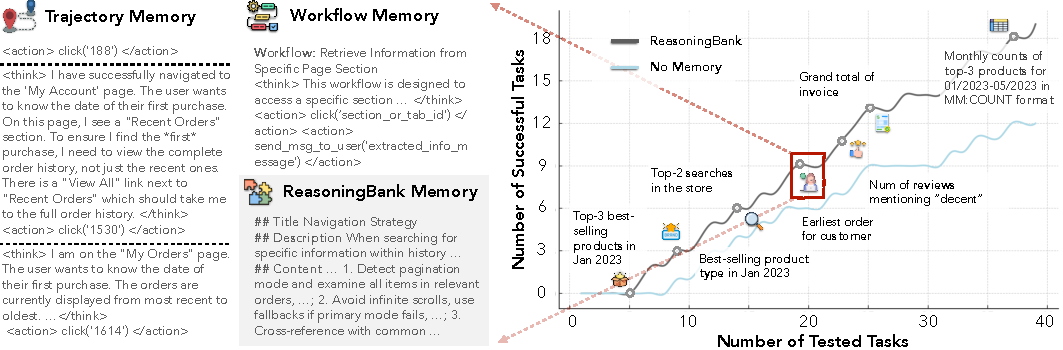
\includegraphics[width=\textwidth]{figures/intro.pdf}
\end{center}
% \vspace{-5mm}
\caption{\ours{} induces reusable reasoning strategies, making memory items more transferable for future use. This enables agents to continuously evolve and achieve higher cumulative success rates than the ``No Memory'' baseline on the WebArena-Admin subset.
}
\label{fig: intro}
% \vspace{-5mm}
\end{figure}

To bridge this gap, we propose \textbf{\ours{}}, a novel memory framework for agent systems.
\ours{} distills and organizes memory items from \textit{both successful and failed experiences} judged by the agent itself without ground-truth labels.
As shown in Figure~\ref{fig: intro}, it captures not only effective strategies from successes but also crucial preventative lessons from failures, abstracting them into a collection of actionable principles.
This process operates in a closed loop: when facing a new task, the agent retrieves relevant memories from \ours{} to guide its actions. Afterward, the new experience is analyzed, distilled, and consolidated back into the \ours{}, allowing the agent to continuously evolve and improve its strategic capabilities.

With \ours{} as a strong experience learner, we study experience scaling to establish a powerful \textbf{synergy between memory and test-time scaling}.
Instead of scaling experience through breadth by adding more tasks, we focus on scaling experience through depth by tackling each single task with more exploration.
We introduce memory-aware test-time scaling (\textbf{\mats{}}) in both parallel and sequential settings, which generates diverse exploration to provide contrastive signals, enabling \ours{} to synthesize better memories.
It creates a synergy between memory and test-time scaling: high-quality memory steers the scaled exploration toward more promising paths, while the rich experiences generated forge even stronger memories.
This positive feedback loop positions \textbf{memory-driven experience scaling} as a new scaling dimension for agents.

We conduct extensive experiments on challenging benchmarks for web browsing (WebArena, Mind2Web) and software engineering (SWE-Bench-Verified). We demonstrate that \ours{} outperforms baselines in both effectiveness (up to 20\% relative improvement, Table~\ref{table: webarena}) and efficiency (up to 16\% fewer interaction steps, Table~\ref{table: webarena}). Additionally, \ours{} synergizes best with \mats{}, making it an essential component for memory-driven experience scaling.

Our contributions are threefold: (1) We propose \ours{}, a novel memory framework that distills generalizable reasoning strategies from both successful and failed experiences, beyond prior work that primarily stores raw trajectories or success-only routines. (2) We introduce \mats{} that establishes a powerful, bidirectional synergy between memory and test-time scaling, with memory-driven experience as a new scaling dimension. (3) We conduct extensive experiments on web browsing (WebArena, Mind2Web) and software engineering (SWE-Bench-Verified) tasks. We demonstrate that our approaches not only outperform baselines in effectiveness (up to 20\% relative improvement) and efficiency (up to 16\% fewer interactions), but also uniquely learn from failures and enable agents to develop increasingly complex, emergent reasoning strategies over time.